\documentclass[8pt]{beamer}
\usetheme{default} % Very simple theme
\usecolortheme{dove} % Minimalist grayscale colors
\setbeamertemplate{navigation symbols}{} % Remove navigation bar

% Define brand-like colors
\definecolor{myblue}{RGB}{0, 102, 204}    % Blue for standard blocks
\definecolor{mygreen}{RGB}{0, 153, 0}     % Green for example blocks
\definecolor{myred}{RGB}{204, 0, 0}       % Red for alert blocks
\definecolor{myorange}{RGB}{255, 128, 0} % For \emph

% Accent color for titles, bullets, etc.
\setbeamercolor{structure}{fg=myblue}

% Block colors
\setbeamercolor{block title}{bg=myblue, fg=white}
\setbeamercolor{block body}{bg=blue!5, fg=black}

\setbeamercolor{exampleblock title}{bg=mygreen, fg=white}
\setbeamercolor{exampleblock body}{bg=green!5, fg=black}

\setbeamercolor{alertblock title}{bg=myred, fg=white}
\setbeamercolor{alertblock body}{bg=red!5, fg=black}
\setbeamercolor{alerted text}{fg=myred}

% Optional: color for \example text
\setbeamercolor{example text}{fg=mygreen}

% Custom emph (orange text instead of italic)
\let\oldemph\emph
\renewcommand{\emph}[1]{\textcolor{myorange}{#1}}


\usepackage{graphicx} % Package for images
\usepackage{amsmath} % Package for images
\graphicspath{{figs/}} % Path to your figures directory
\usepackage{array}  % For better column spacing
\usepackage{caption} % Required for \captionof

% Title Information
\title{STOCHASTIC METHODS IN WATER RESOURCES}
\vspace{25pt}
\subtitle{Unit 3: Random functions \\ Lecture 9: Definitions, random function types, stationary random functions}
\author{Luis Alejandro Morales, Ph.D.}
\institute{Universidad Nacional de Colombia \\ Department of Civil and Agriculture Engineering} %// }
%\date{\today}

\begin{document}

% Title Slide
\begin{frame}
    \titlepage
\end{frame}

%-------
% From Bierke
\section{Definitions}
\begin{frame}{Definitions}
    \begin{itemize}
        \item Consider a \emph{hydrological variable} $Z$ that can either varies in space (e.g. hydraulic conductivity) or in time (e.g. surface water level) or in space and time (e.g. growndwater depth). 
        \item The value of any of these variables is known only in those places where it is observed, and it is unknown in other places. 
        \item Accordingly, the value of $Z$ is uncertain, to deal with this, instead of using one single functio either in time ($Z(t)$), or space ($Z(\mathbf{x})$) or space and time ($Z(\mathbf{x},t)$), multiple functions are used (see figure for $Z(t)$).  
        \item Each of these functions have the same probability of representing the true. 
        \item The family of equally probable functions representing $Z$ is known as an \alert{emsemble} or a \alert{random function}. 

    \end{itemize}

\centering
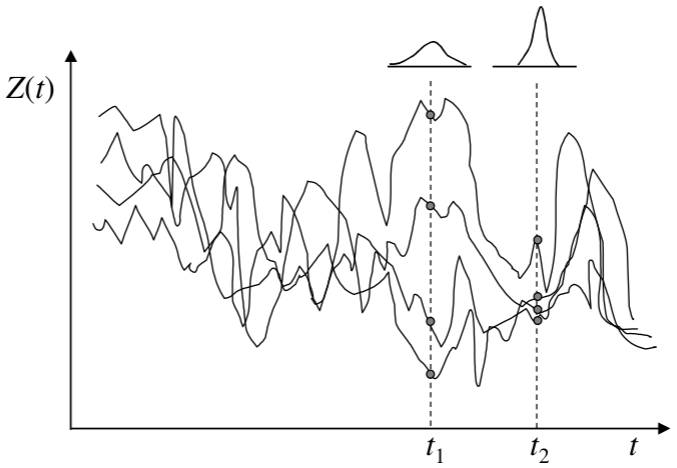
\includegraphics[width=0.7\linewidth]{fiBi51.png}  % from Bierk

\end{frame}

\begin{frame}{Definitions}
    \begin{itemize}
        \item \alert{Random field}: If $Z$ is a function of space ($\mathbf{x}$), $Z(\mathbf{x})$, $\mathbf{x}= (x,y, z)$. 
        \item \alert{Random or stochastic process}: If $Z$ is a function of time ($t$), $Z(t)$.
        \item \alert{Space-time random field}: If $Z$ is a function of space ($\mathbf{x}$) and time ($t$), $Z(\mathbf{x},t)$, $\mathbf{x}= (x,y, z)$.
   \end{itemize}
   Here, we are going to focus on \emph{random process} ($Z(t)$). Note that in the figure above, four functions $Z(t)$ (\emph{ensemble members}) are shown and each of them are know as \emph{realizations} and denoted as $z(t)$. The number of \emph{realizations}, depending on the variable's nature, can be finite or infinite.\\ 

   Another way of explaining this concept is to imagine a \emph{random function} as a collection of random variables (one at every location in space or point in time). Observing at the figure above, for each time $t$, a $Z(t)$ is defined. This is why for each $t$, $Z(t)$ is described with a \emph{pdf} $f_Z (z; t)$, which depends not only on the value of $z$ but also on the value of $t$. These \emph{pdf} is estimated based on sample of data taken at particular time (e.g. $t_1$). As shown in the figure, the \emph{pdf}s of the data sample at $t_1$ and $t_2$ are different, and indicate that variance is larger in $t_1$ than in $t_2$ and thus more uncertain. \\

   At each point in time ($t$), $\mu_Z$ is calculated as:
   \[
       \mu_Z (t) = E[Z(t)] = \int_{-\infty}^{\infty} z f_Z (z; t) dz
   \]
   and $\sigma_Z^2$ is:
   \[
       \sigma_Z^2 (t) = E[(Z(t)-\mu_Z (t))^2] = \int_{-\infty}^{\infty} (z-\mu_Z (t))^2 f_Z (z; t) dz
   \]

\end{frame}

\begin{frame}{Definitions}
    The \emph{random variables} are usually correlated in time (or in space for spatial random functions). This means that the \emph{covariance} $COV[Z(t_1), Z(t_2)] \neq 0$. Note that the  further apart the points (e.g. $t_1$ and $t_2$) the lower the \emph{covariance}. This is estimated as
    \begin{align*}
        COV[Z(t_1), Z(t_2)]  &= E[(Z(t_1)-\mu_Z (t_1))(Z(t_2)-\mu_Z (t_2))] \\
                             &= \int_{-\infty}^{\infty} \int_{-\infty}^{\infty} (z_1-\mu_{Z}(t_1)) (z_2-\mu_{Z}(t_2)) f_Z (z_1, z_2; t_1, t_2) dz_1 dz_2
    \end{align*}
    if $t_1 = t_2$, $COV[Z(t_1), Z(t_2)]  = \sigma_Z^2 (t)$. \\

    For $n$ different locations $t_i$ where $i=1, 2, \cdots, n$, the probability measure that a realization of $Z(t)$ has the values between $z_1 < z(t_1) \leq z_1 + dz_1$, $z_2 < z(t_2) \leq z_2 + dz_2$, $\cdots$, $z_n < z(t_n) \leq z_n + dz_n$. The \emph{associated multivariate pdf} $f_{Z(t_1), Z(t_2),\cdots,Z(t_n)} (z_1, z_2, \cdots, z_n; t_1, t_2, \cdots, t_n)$
    \begin{align*}
        &f_{Z(t_1), Z(t_2),\cdots,Z(t_n)} (z_1, z_2, \cdots, z_n; t_1, t_2, \cdots, t_n) = \\ 
                                                                                        &\lim_{\partial z_1, \cdots, \partial z_n \rightarrow 0} \frac{Pr(z_1 < z(t_1) \leq z_1 + \partial z_1, z_2 < z(t_2) \leq z_2 + \partial z_2, \cdots, z_n < z(t_n) \leq z_n + \partial z_n)}{\partial z_1 \partial z_2 \cdots \partial z_n}
    \end{align*}
    The \emph{multivariate pdf} of a \emph{random function} is sometime referred to as \alert{multipoint pdf}, because it relates to random variables at different points or locations. Note that \emph{random function} is fully characterized if the \emph{multivariate pdf} for any set of points is known. 

\end{frame}

%-------
% From Bierke
\section{Types of random functions}
\begin{frame}{Types of random functions}
    \emph{Random functions} can be classified as \emph{continuous} whether the \emph{random variable} is continuous (e.g. maximum annual river flows) or \emph{discrete} whether the \emph{random variable} is discrete (e.g. number of annual rainy days). Other way to classify a random function is based its domain (see figure). In the case of a \emph{continuous random function}, this can be defined at:
    \begin{enumerate}

        \item \emph{all locations} in time, space or space-time: $Z(t)$, $Z(\mathbf{x})$ or $Z(\mathbf{x},t)$.
        \item \emph{discrete points} in time, space or space-time, where $Z(k\Delta t)$ ($k=1,2,\cdots,K$) is referred to as a \alert{random time series}, and $Z(i\Delta x, j\Delta y)$ ($i=1,2,\cdots, I$; $j=1,2,\cdots, J$) as a \alert{lattice process}.
        \item \emph{random times} or \emph{random locations} is space and time: $Z(T)$, $Z(\mathbf{X})$ or $Z(\mathbf{X},T)$. This process is called \alert{compound point process}. Note that the occurrence of the points at random coordinates in space and time is called a \alert{point process}. If the occurrence of such a point is associated with the occurrence of a random variable (e.g. the occurrence of a thunder storm cell at a certain location in space with a random intensity of rainfall) it is called a compound point process.
    \end{enumerate}

    The same distinction can be made for discrete-valued random functions: $D(t)$, $D(k\Delta t)$ or $D(T)$; $D(\mathbf{x})$, $D(i\Delta x, j\Delta y)$ or $D(\mathbf{X})$. 

\end{frame}

\begin{frame}{Types of random functions}

    \begin{center}
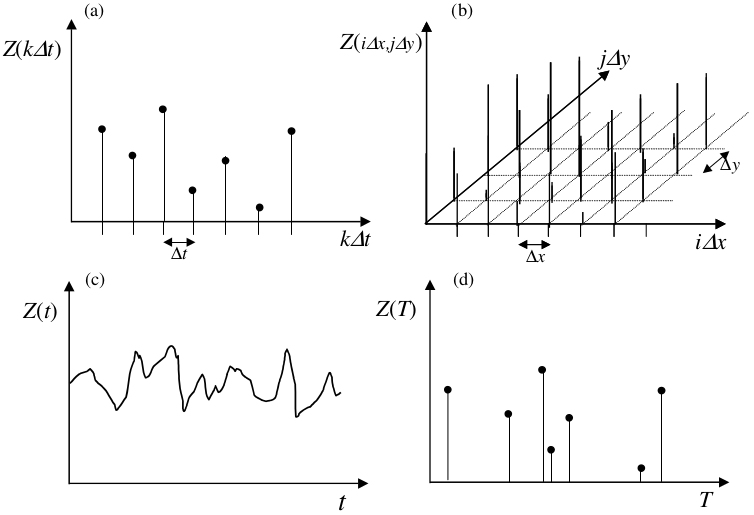
\includegraphics[width=0.9\linewidth]{fiBi52.png}  % from Bierk
    \end{center}

This figure shows the different types of \emph{random functions} based on the way they are defined on the functional domain: a) random time series, b) lattice process, c) continuous-time random function and d) compound point process. 
\end{frame}

%-------
% From Bierke
\section{Stationary random functions}
\begin{frame}{Stationary random functions}
    \begin{block}{Strict stationary random functions}
    \end{block}
    An special type of random functions are the \alert{strict stationary random functions}. A \emph{strict stationary random functions} isa random function for which its \emph{multivariate pdf} is invariant under translation. This means that for any set of $N$ locations and for any translations in time $\Delta t$, we have
    \begin{align*}
        f(z_1, z_2, \cdots, z_N ; t_1, t_2, \cdots, t_N ) &= \\
                                                          &f(z_1, z_2, \cdots, z_N ; t_1 +\Delta t, t_2+\Delta t, \cdots, t_N +\Delta t)  \quad \forall t_i, \Delta t
    \end{align*}


\begin{minipage}[]{0.48\textwidth}
    This assume that a configuration of points on the time axis can move backward and forward in time and the \emph{multivariate pdf} does not change. For the spatial domain, \emph{strict stationarity} means spatial no changes in the \emph{pdf} if points are translated but no rotated. For instance a \emph{strict random function} in 2D (see figure) the two sets of locations in the left-hand figure have the same \emph{multivariate pdf}, while the locations in the right-hand figure necessarily does not. If the \emph{multivariate pdf} of the \emph{random function} is invariant under rotation, this is called a \alert{statistically isotropic random function}.     
\end{minipage}
%\hfill
\begin{minipage}[]{0.48\textwidth}
    \centering
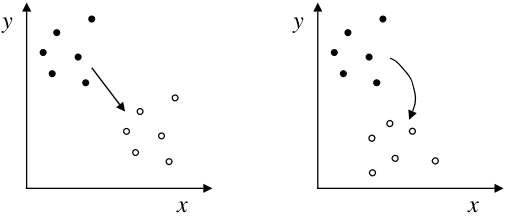
\includegraphics[width=\linewidth]{fiBi53.png}  % from Bierk
\end{minipage}

\end{frame}

\begin{frame}{Stationary random functions}
    \begin{block}{Ergodic random functions}
    \end{block}
    \begin{itemize}
        \item To estimate the statistical properties of a \emph{random function}, a large number of realizations must be drew. 
        \item This is the case, for instance, of throwing a dice, from where one can generate multiple realizations. 
        \item In reality this is not possible because we only have one realization: \emph{reality}. This means that all relevant statistics of the \emph{random function} are estimated from a single realization. 
        \item In general, \alert{ergodicity} deal with \emph{stationarity} in \emph{random functions}. 
        \item To analyse \emph{ergodicity}, statistical properties such as the \emph{mean}, the \emph{standard deviation} and the \emph{covariance} are examined.  
        \item \emph{Stationarity} tells that all these properties are invariant no matter where you are (e.g. in time). 
        \item For instance, for multiple realizations at point $t_1$ of $Z(t)$, the normal procedure to compute  $\mu_Z (t_1)$ would be to average these realizations. However, this is impossible because in reality we only have one realization.
        \item If the \emph{random function} is stationary the \emph{pdf} $f_Z (z; t)$ at any location (in time) is the same and thus the statistical properties. 
        \item This also means that within any single realisation we have at every location a sample from the same \emph{pdf} $f_Z (z;t)$. 
    \end{itemize}

\end{frame}

\begin{frame}{Stationary random functions}
    \begin{block}{Ergodic random functions}
    \end{block}
    \begin{itemize}
        \item So, the \emph{mean} can also be estimated if we take a sufficient number of samples from a single realisation, such as our \emph{reality} (see figure below)

            \begin{center}
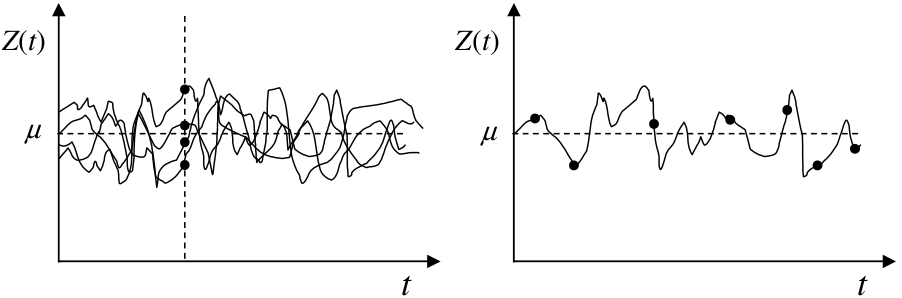
\includegraphics[width=\linewidth]{fiBi54.png}  % from Bierk
            \end{center}
        \item This property of a \emph{random function}, i.e. being able to estimate statistical properties of a random function from a large number of samples of a \emph{single realisation} is called \alert{ergodicity}.
        \item So for a \emph{random function} is \alert{ergodic} if it is \emph{stationary}.
        \item Also for a \emph{random function} to be \emph{ergodic},  the samples from the single realisation should be taken from a large enough period of time or, in the spatial case, large enough area. 
    \end{itemize}
    
\end{frame}

\begin{frame}{Stationary random functions}
    \begin{block}{Ergodic random functions}
    \end{block}
    A formal definition of \emph{ergodicity} of a \emph{random function} in its \emph{mean}
    \[
    \lim_{T\rightarrow \infty} \frac{1}{T} \int_T z(t) dt = \int_{-\infty}^{\infty} z f_Z (z;t) dz = \mu_Z
\]
where $T$ is an interval of time. This equation means that  the integral over the probability distribution (the ensemble) for a given $t$ (term on the left)  can be replaced by a temporal (or spatial or spatio-temporal) integral of a very large interval $T$ (or area or volume) (term on the right) to estimate $\mu_Z$. 
volume).

Similarly, \emph{ergodicity} of a \emph{random function} in its \emph{mean} is defined as
\begin{align*}
    \lim_{T\rightarrow \infty} \frac{1}{T^2} \int_T z(t) z(t+\tau) dt &= \int_{-\infty}^{\infty} \int_{-\infty}^{\infty} (z_1 -\mu_Z) (z_2 -\mu_Z)  f(z_1, z_2;t, t+\tau) dz_1 dz_2  \\
    &= COV[Z(T), Z(t+\tau)] \quad \quad \forall \tau
\end{align*}
where $\tau$ is delta time. 

\end{frame}

 \begin{frame}{Stationary random functions}
     \begin{block}{Second order stationary random functions}
    \end{block}
    A weaker form of \emph{stationarity} is second order \emph{stationarity}. This means that  the bivariate (or two-point) \emph{probability distribution} is invariant under translation 
    \[
    f(z_1, z_2; t_1, t_2) = f(z_1, z_2; t_1 + \tau, t_2+\tau) \quad \quad \forall t_1 , t_2, \tau 
\]
In practice, one require only \emph{ergodicity} and thus \emph{stationarity} for the \emph{mean}, \emph{varianza} and \emph{covariance}. An \emph{milder stationarity} is even considered and called \alert{weak sense stationarity}. For \emph{wide sense stationary random functions}
\begin{align*}
    \mu_Z (t) &= \mu_Z \quad \text{constant and $t$ or $\mathbf{x}$ independent}\\
    \sigma_Z (t) &= \sigma_Z \quad \text{constant and $t$ or $\mathbf{x}$ independent}\\
    COV[Z(t_1) Z(t_2)] &= C_Z(t_2 - t_1) = C_Z (\tau) \quad \text{depends on $\tau$ (separation in time or space)}
\end{align*}
The \alert{covariance function} is a graph that describe the covariance and depends on $\tau$ (\alert{lag}). The covariance function start when $t_1 = t_2$ (variance of both variables) and when $\tau$ increase the function tends to zero. This means that a random variable is not correlated for larger $\tau$.

In the case of \emph{random space functions} the \emph{weak sense stationarity} means that $COV [Z(\mathbf{x}_1), Z(\mathbf{x}_2)] = C_Z (\mathbf{x}_2 - \mathbf{x}_1) = C_Z (\mathbf{h})$, where $\mathbf{h} = \mathbf{x}_2 - \mathbf{x}_1$. In case of a \emph{isotropic} random function $COV [Z(\mathbf{x}_1), Z(\mathbf{x}_2)] = C_Z (|\mathbf{x}_2 - \mathbf{x}_1|) = C_Z (\mathbf{|h|}) = C_Z (h)$, where $|\mathbf{h}|=h$ is the \emph{norm} of the difference vector. 
\end{frame}
 
 \begin{frame}{Stationary random functions}
     \begin{block}{Second order stationary random functions}
    \end{block}
    When the \emph{covariance function} is divided by the \emph{variance} $\sigma_Z^2$, this becomes the \alert{correlation function} either $\rho_Z(\tau) = C_Z(\tau)/\sigma_Z^2$ or $\rho_Z(\mathbf{h}) = C_Z (\mathbf{h})/\sigma_Z^2$. When the data is regularly spaced either in time or space, the \emph{covariance function} is:
    \[
        \hat{C}_Z(k\Delta t) =  \frac{1}{n-k} \sum_{k=1}^{n-k} (z_i - \hat{\mu}_Z ) (z_{i+k} - \hat{\mu}_Z )
    \]
    where $k\Delta t$ is the lag (in units of time or space) and $\Delta t$ is the distance (in time or space) between observations. Frequently the estimator $\hat{C}_Z (k\Delta t)$ is used in the analysis of time series. In the case of irregularly positioned data in space, the \emph{covariance function} is
    \[
        \hat{C}_Z(\mathbf{h}) =  \frac{1}{n(\mathbf{h})} \sum_{i=1}^{n(\mathbf{h})} (z(\mathbf{x_i}) - \hat{\mu}_Z ) (z(\mathbf{x_i}+ \mathbf{h} \pm \mathbf{\Delta h}) - \hat{\mu}_Z ) 
    \]
where $\mathbf{h}$ is the lag (a vector in space), $\Delta \mathbf{h}$ is a lag-tolerance  which is needed to group a number of data-pairs together  to get stable estimates for a given lag and $n(\mathbf{h})$ are the number of data pairs that are a distance $\mathbf{h} \pm \Delta \mathbf{h}$ apart. 

\end{frame}

 \begin{frame}{Stationary random functions}
     \begin{exampleblock}{Correlation function: maximum annual streamflow}
\begin{minipage}[]{0.48\textwidth}
    \centering
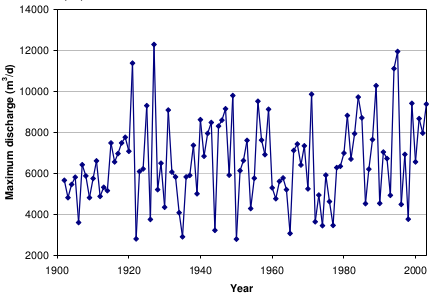
\includegraphics[width=\linewidth]{fiBi56a.png}  % from Bierk
\end{minipage}
\begin{minipage}[]{0.48\textwidth}
    \centering
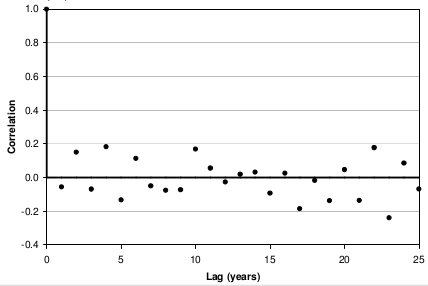
\includegraphics[width=\linewidth]{fiBi56b.png}  % from Bierk
\end{minipage}
     \end{exampleblock}
     \begin{itemize}
         \item The correlation plot, shows the \emph{estimated} and the \emph{fitted} correlation functions. According to these plots the data is uncorrelated.
         \item This uncorrelated behaviour of lagged data points is a characteristics of \alert{white noise}, which are pure random processes, where the data points are uncorrelated no matter $\tau$. 
         \item \emph{White noise} follow a \emph{normal distribution}, so that, one can produce synthetic e.g. annual maximum streamflows after sampling the process. It would produce a time series with the same statistical properties of the original one.  
     \end{itemize}
\end{frame}

 \begin{frame}{Stationary random functions}
     \begin{exampleblock}{Correlation function: daily water table depth (1994-1995)}
\begin{minipage}[]{0.48\textwidth}
    \centering
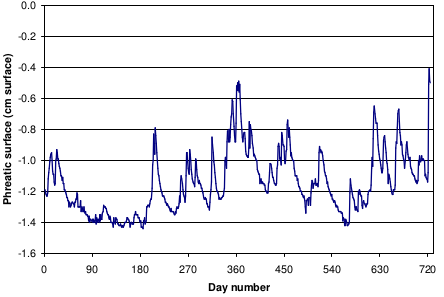
\includegraphics[width=\linewidth]{fiBi56d.png}  % from Bierk
\end{minipage}
\begin{minipage}[]{0.48\textwidth}
    \centering
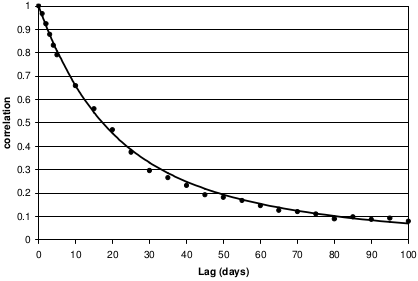
\includegraphics[width=\linewidth]{fiBi56e.png}  % from Bierk
\end{minipage}
     \end{exampleblock}
     \begin{itemize}
         \item The correlation plot, shows the \emph{estimated} and the \emph{fitted} correlation functions. According to these plots the correlation decrease exponentially as $\tau$ increase. 
         \item Again,  one can produce synthetic e.g. daily water  levels after sampling the process at the same discrete times. It would produce a time series with the same statistical properties of the original one.  
     \end{itemize}
\end{frame}

 \begin{frame}{Stationary random functions}
     \begin{block}{Second order stationary random functions}
    \end{block}

    The following table shows some models for modelling the \emph{covariance function} for \emph{isotropic random functions} and  \emph{wide sense stationary process}. 

    \begin{center}
  \begin{tabular}{|l|c|}
    Exponential covariance & $C_Z (h) = \sigma_Z^2 e^{-h/a}$ for $h\geq 0$, $a>0$ \\ 
    Gaussian covariance         & $C_Z (h) =  \sigma_Z^2  e^{-h^2/a^2}$  for $h\geq 0$, $a>0$ \\ 
    Spherical covariance         & \[ C_Z (h) = \left\{ \begin{array}{l}  \sigma_Z^2 \left[ 1 - \frac{3}{2}\left(\frac{h}{a}\right) + \frac{1}{2}\left(\frac{h}{a}\right)^3 \right]   \text{, if } h< a  \\ 0 = \text{, if } h\geq a, h\geq 0, a>0 \end{array} \right. \] \\ 
    Hole effect (wave) model & $C_Z (h) = \sigma_Z^2 \frac{b\sin (h/a)}{h}$ for $h\geq 0$, $a>0$ \\ 
    White noise model &  \[ \rho_Z (h) = \left\{ \begin{array}{l}  1 \text{, if } h=0  \\ 0 = \text{, if } h>0 \end{array} \right. \] \\ 

  \end{tabular}
    \end{center}
    Note that the \emph{white noise model} has infinity variance, so it is not \emph{wide sense stationary}. 
     \begin{block}{Relations between various forms of stationarity}
    \end{block}
    If a \emph{random function} is \emph{wide sense stationary} and its \emph{multivariate pdf} is a \emph{Gaussian distribution}, It is also second order stationary and also a strict sense \emph{stationary random function}. More important, a wide sense stationary random function that is multivariate Gaussian (and thus also strict stationary) is completely characterised by only a few statistics:  a constant \emph{mean} $\mu_Z (t) = \mu_Z$  and a \emph{covariance  function} $C_Z (t_2 - t_1)$ that only depends on the separation distance. 


\end{frame}

 \begin{frame}{Stationary random functions}
     \begin{block}{Intrinsic random functions}
         For an intrinsic random function we require (we show the spatial form here) $E[Z(\mathbf{x_2}) - Z(\mathbf{x_1}) ] = 0$ $\forall \mathbf{x_2}, \mathbf{x_1}$
    \end{block}
\end{frame}


\end{document}
